\documentclass[aspectratio=169,10pt]{beamer}

\usepackage[T1]{fontenc}
\usepackage[utf8]{inputenc}
\usefonttheme{professionalfonts}
\usepackage{amsmath,amssymb,mathtools,bm}
\usepackage{booktabs,tabularx,array,multirow,makecell,colortbl}
\usepackage{graphicx}
\usepackage{ragged2e}
\usepackage{microtype}
\usepackage{appendixnumberbeamer}

\graphicspath{%
  {assets/}%
  {../thesis_phd_math/images/ch2/}%
  {../thesis_phd_math/images/ch3/}%
  {../thesis_phd_math/images/ch4/}%
}
% Visual language adapted from the two supplied defense presentations:
% a restrained blue academic layout, a strong title rule, compact footer,
% and contribution ribbons linking results to the specialty passport.

\definecolor{IUBlue}{RGB}{13,88,148}
\definecolor{IUDeepBlue}{RGB}{8,55,101}
\definecolor{IULightBlue}{RGB}{232,242,250}
\definecolor{IUPaleBlue}{RGB}{246,250,253}
\definecolor{GapRed}{RGB}{184,45,54}
\definecolor{GapPale}{RGB}{251,237,239}
\definecolor{ContributionGreen}{RGB}{31,126,93}
\definecolor{ContributionPale}{RGB}{231,246,240}
\definecolor{ConstraintOrange}{RGB}{220,124,32}
\definecolor{ConstraintPale}{RGB}{253,243,230}
\definecolor{Ink}{RGB}{24,31,42}
\definecolor{MidGray}{RGB}{90,99,112}
\definecolor{RuleGray}{RGB}{190,198,207}
\definecolor{SoftGray}{RGB}{244,246,248}

\setbeamercolor{normal text}{fg=Ink,bg=white}
\setbeamercolor{structure}{fg=IUBlue}
\setbeamercolor{frametitle}{fg=Ink,bg=white}
\setbeamercolor{title}{fg=white,bg=IUBlue}
\setbeamercolor{subtitle}{fg=white,bg=IUBlue}
\setbeamercolor{itemize item}{fg=IUBlue}
\setbeamercolor{itemize subitem}{fg=IUBlue}
\setbeamercolor{enumerate item}{fg=white,bg=IUBlue}
\setbeamercolor{block title}{fg=white,bg=IUBlue}
\setbeamercolor{block body}{fg=Ink,bg=IUPaleBlue}
\setbeamercolor{alerted text}{fg=GapRed}
\setbeamercolor{claimbar}{fg=IUDeepBlue,bg=IULightBlue}

\setbeamerfont{title}{size=\Large,series=\bfseries}
\setbeamerfont{subtitle}{size=\normalsize}
\setbeamerfont{frametitle}{size=\Large,series=\mdseries}
\setbeamerfont{footline}{size=\scriptsize}
\setbeamerfont{block title}{series=\bfseries}

\setbeamersize{text margin left=0.55cm,text margin right=0.55cm}
\setbeamertemplate{navigation symbols}{}
\setbeamertemplate{itemize item}{\raise0.15ex\hbox{\color{IUBlue}\small$\bullet$}}
\setbeamertemplate{itemize subitem}{\raise0.12ex\hbox{\color{IUBlue}\scriptsize$\blacktriangleright$}}
\setbeamertemplate{enumerate item}{%
  
\begin{tikzpicture}[baseline=(n.base)]
    \node[circle,fill=IUBlue,inner sep=1.25pt,text=white,font=\bfseries\scriptsize] (n) {\insertenumlabel};
  \end{tikzpicture}%
}

\setbeamertemplate{frametitle}{%
  \nointerlineskip
  \begin{beamercolorbox}[wd=\paperwidth,ht=0.78cm,dp=0.22cm,leftskip=0.55cm,rightskip=0.45cm]{frametitle}%
    \usebeamerfont{frametitle}\insertframetitle
    \hfill
    \raisebox{-0.05ex}{%
      
\begin{tikzpicture}[baseline=(brand.base)]
        \node[draw=IUBlue,line width=0.45pt,inner xsep=4pt,inner ysep=2pt,
          text=IUBlue,font=\bfseries\tiny] (brand) {INNOPOLIS UNIVERSITY};
      \end{tikzpicture}}
  \end{beamercolorbox}%
  \nointerlineskip
  \begin{beamercolorbox}[wd=\paperwidth,ht=0.075cm,dp=0cm]{title rule}\end{beamercolorbox}%
}
\setbeamercolor{title rule}{bg=IUBlue}

\setbeamertemplate{footline}{%
  \leavevmode
  \hbox{%
    \begin{beamercolorbox}[wd=.36\paperwidth,ht=0.30cm,dp=0.13cm,leftskip=0.55cm]{footline}%
      \color{MidGray}\insertshortauthor
    \end{beamercolorbox}%
    \begin{beamercolorbox}[wd=.38\paperwidth,ht=0.30cm,dp=0.13cm,center]{footline}%
      \color{MidGray}Innopolis, 2026
    \end{beamercolorbox}%
    \begin{beamercolorbox}[wd=.26\paperwidth,ht=0.30cm,dp=0.13cm,rightskip=0.55cm plus 1fil]{footline}%
      \color{MidGray}\insertframenumber\,/\,\inserttotalframenumber
    \end{beamercolorbox}%
  }
}

\setbeamertemplate{blocks}[rounded][shadow=false]

\tikzset{
  flowbox/.style={
    draw=IUBlue, line width=0.7pt, rounded corners=2pt,
    fill=IUPaleBlue, align=center, inner sep=4pt,
    minimum height=0.75cm, font=\small
  },
  contribution/.style={
    draw=ContributionGreen, line width=0.8pt, rounded corners=2pt,
    fill=ContributionPale, align=center, inner sep=4pt,
    minimum height=0.78cm, font=\small
  },
  gapbox/.style={
    draw=GapRed, line width=0.8pt, rounded corners=2pt,
    fill=GapPale, align=center, inner sep=4pt,
    minimum height=0.78cm, font=\small
  },
  constraintbox/.style={
    draw=ConstraintOrange, line width=0.8pt, rounded corners=2pt,
    fill=ConstraintPale, align=center, inner sep=4pt,
    minimum height=0.78cm, font=\small
  },
  processarrow/.style={-{Latex[length=2.0mm,width=1.4mm]},line width=0.8pt,draw=IUBlue},
  rejectarrow/.style={-{Latex[length=1.9mm,width=1.35mm]},line width=0.7pt,draw=GapRed,dashed},
  tinylabel/.style={font=\scriptsize,text=MidGray,align=center}
}

\newcommand{\source}[1]{%
  \par\vspace{0.8mm}{\color{MidGray}\scriptsize Source: #1\par}%
}

\newcommand{\claimbar}[2]{%
  \vfill
  \begin{beamercolorbox}[wd=\textwidth,sep=2.0pt,left]{claimbar}%
    \fontsize{5.9}{6.8}\selectfont
    \parbox[t]{0.755\textwidth}{\raggedright\textbf{#1}}\hfill%
    \parbox[t]{0.205\textwidth}{\raggedleft #2}
  \end{beamercolorbox}%
}

\newcommand{\metriccard}[3][IUBlue]{%
  \begin{tikzpicture}[baseline=(m.base)]
    \node[draw=#1,line width=0.65pt,rounded corners=2pt,fill=#1!7,
      text width=2.75cm,minimum height=1.25cm,align=center,inner sep=3pt] (m) {%
      {\color{#1}\bfseries\Large #2}\\[-0.2ex]
      {\footnotesize #3}};
  \end{tikzpicture}%
}

\newcommand{\smalltag}[2][IUBlue]{%
  \tikz[baseline=(t.base)]\node[draw=#1,rounded corners=1.5pt,fill=#1!7,
    text=#1,inner xsep=3pt,inner ysep=1.5pt,font=\bfseries\footnotesize] (t) {#2};%
}

\newcommand{\takeaway}[1]{%
  \begin{beamercolorbox}[wd=\textwidth,sep=4pt,left]{claimbar}%
    \small\textbf{Takeaway:} #1
  \end{beamercolorbox}%
}


\title[Mathematical modeling and motion planning]{%
  Mathematical Modeling and Motion Planning\\
  for Robotic Manipulation of Deformable Linear Objects}
\author[Karam Almaghout]{Karam Almaghout}
\institute{Innopolis University}
\date{Innopolis, 2026}

\hypersetup{
  pdftitle={Mathematical Modeling and Motion Planning for Robotic Manipulation of Deformable Linear Objects},
  pdfauthor={Karam Almaghout},
  colorlinks=true,
  linkcolor=IUBlue,
  urlcolor=IUBlue
}

\newcommand{\R}{\mathbb{R}}
\newcommand{\Cfree}{\mathcal C_{\mathrm{free}}}
\newcolumntype{Y}{>{\RaggedRight\arraybackslash}X}
\newcolumntype{C}[1]{>{\Centering\arraybackslash}p{#1}}

\begin{document}

% =============================================================================
% 1. Title
% =============================================================================
\begin{frame}[plain]
  \vspace*{0.52cm}
  {\color{IUBlue}\rule{\textwidth}{1.0pt}}\par
  \vspace{0.45cm}
  {\usebeamerfont{title}\color{Ink}\inserttitle\par}
  \vspace{0.25cm}
  {\color{IUBlue}\rule{0.28\textwidth}{2.2pt}}\par

  \vspace{0.70cm}
  \begin{tabular}{@{}p{4.1cm}p{8.5cm}@{}}
    \textbf{Candidate} & Karam Almaghout\\[0.28cm]
    \textbf{Scientific supervisor} & Alexandr Klimchik, PhD\\[0.28cm]
    \textbf{Organization} & Innopolis University\\[0.28cm]
    \textbf{Specialty 1.2.2} &
      Mathematical modeling, numerical methods and software packages
  \end{tabular}

  \vfill
  \begin{flushright}
    \color{MidGray}Thesis for the degree of Candidate of Technical Sciences
    % Innopolis, 2026
  \end{flushright}
\end{frame}

% =============================================================================
% 2. Relevance
% =============================================================================
\begin{frame}[t]{Relevance and applications}
  \begin{columns}[T,onlytextwidth]
    \begin{column}{0.42\textwidth}
      \centering
      
\includegraphics[width=0.93\linewidth,height=2.25cm,keepaspectratio]{wire_harness.jpg}\\[-0.2ex]
      {\footnotesize Wire-harness assembly}

      \vspace{0.15cm}
      
\includegraphics[width=0.93\linewidth,height=2.05cm,keepaspectratio]{surgical_threads.png}\\[-0.2ex]
      {\footnotesize Surgical-thread manipulation}
    \end{column}

    \begin{column}{0.56\textwidth}
      \small
      A \textbf{deformable linear object (DLO)} is a cable, wire, rope,
      hose, or thread whose complete shape changes during manipulation.

      \vspace{0.25cm}
      \begin{itemize}
        \item A DLO has distributed compliance and effectively many degrees of
          freedom; its endpoints do not determine its shape.
        \item Material and dynamic parameters are difficult to identify for
          every object.
        \item Collision-free gripper paths do not guarantee a collision-free
          motion of the complete cable.
      \end{itemize}

      \vspace{0.20cm}
      \textbf{Research question.} How can two robots deform and route a
      planar DLO using its observed geometry, without prior identification of
      stiffness or damping?
    \end{column}
  \end{columns}

  % \source{Dissertation, Introduction, pp.~7--39.}
\end{frame}

% =============================================================================
% 3. Literature and gap
% =============================================================================
\begin{frame}[t]{Existing approaches and the research gap}
  \small
  \renewcommand{\arraystretch}{1.28}
  \setlength{\tabcolsep}{5pt}
  \begin{tabularx}{\textwidth}{>{\bfseries}p{2.35cm}YY}
    \toprule
    \tablehead{Approach} & \tablehead{What it provides} &
      \tablehead{Limitations}\\
    \midrule
    Model-free control &
      A local relation between gripper motion and observed cable points. &
      Valid mainly near the current shape; large changes and opposite
      concavity may not be reached.\\
    Model-based control &
      Prediction from a mechanical DLO model. &
      Requires material parameters that are difficult to identify.\\
    Data-driven control &
      A relation learned from examples. &
      Requires representative training data and may not generalize.\\
    Existing routing methods &
      Search over robot poses or isolated cable shapes. &
      Two valid shapes may still be joined by a cable motion that crosses an
      obstacle or reverses endpoint correspondence.\\
    \bottomrule
  \end{tabularx}

  \vspace{0.24cm}
  \textbf{Gap:} one ordered cable
  representation, large-deformation intermediary shapes, local control
  without identified cable parameters, and global routing with complete
  transition validation.

  % \source{Dissertation, Chapter 1 and Introduction.}
\end{frame}

% =============================================================================
% 4. Goal and tasks
% =============================================================================
\begin{frame}[t]{Goal, object, subject, and research objectives}
  \small
  \textbf{Goal.} Develop mathematical models and effective numerical methods
  for dual-arm shape control and routing of DLOs under large planar
  deformations and workspace obstacles, without prior identification of
  dynamic or material parameters.

  \vspace{0.16cm}
  % \begin{columns}[T,onlytextwidth]
  %   \begin{column}{0.31\textwidth}
  %     \footnotesize
  %     \textbf{Object}\\
  %     Planar dual-arm robotic manipulation of DLOs.

  %     \vspace{0.20cm}
  %     \textbf{Subject}\\
  %     Models, numerical methods, and algorithms for representation,
  %     simulation, visual reconstruction, deformation planning, control,
  %     and routing.
  %   \end{column}
  %   \begin{column}{0.67\textwidth}
  %     \footnotesize
      \textbf{Research objectives}
      \begin{enumerate}
        \item Detect and track a marker-free cable in 2D by a single camera.
        \item Generate length-feasible intermediary configurations, including
          opposite-concavity transformations.
        \item Model the local robot--cable kinematics and calculate bounded
          dual-arm motion.
        \item Model the DLO configuration space and plan routes among static
          obstacles with valid swept motion.
        \item Implement and verify the developed models and methods.
      \end{enumerate}
  %   \end{column}
  % \end{columns}

  % \source{Dissertation, Introduction, pp.~59--98.}
\end{frame}

% =============================================================================
% 5. Research map
% =============================================================================
\begin{frame}[t]{Research structure}
  \centering
  \footnotesize
  \renewcommand{\arraystretch}{1.21}
  \setlength{\tabcolsep}{3.5pt}
  \begin{tabularx}{\textwidth}{
    >{\bfseries\RaggedRight\arraybackslash}p{2.05cm}YYY}
    \toprule
    & \tablehead{Perception} &
      \tablehead{Large-deformation shape control} &
      \tablehead{Global cable routing}\\
    \midrule
    Problem &
      Observe a featureless cable as an ordered, fixed-size state. &
      Move between distant shapes, including opposite concavity. &
      Route the complete cable among obstacles.\\
    \addlinespace[1mm]
    Prior limitation &
      Markers require preparation; dense contours increase computation. &
      Local methods, identified models, or training data restrict use. &
      Endpoint or static-shape checks miss swept cable collisions.\\
    \addlinespace[1mm]
    Contributions &
      Virtual Feature Points (VFPs) Agorithm. &
      Angular-linear interpolation (ALI) algorithm;
      diminishing-rigidity Jacobian; control as an optimization problem. &
      Configuration-space global routing; ordered swept-transition test.\\
    \addlinespace[1mm]
    Verification &
      Top-view image detection and tracking. &
      32 simulation tasks and physical experiments with two KUKA robots. &
      10,000 C++ trials and MuJoCo execution with two UR10 robots.\\
    \midrule
    Chapter & \textbf{2} & \textbf{3} & \textbf{4}\\
    \bottomrule
  \end{tabularx}

  \vspace{0.13cm}
  {\scriptsize Chapter 1 provides the systematic analysis and formulates the
  research gap.}
\end{frame}

% =============================================================================
% 6. Provisions
% =============================================================================
% \begin{frame}[t]{Provisions presented for defense}
%   \small
%   \renewcommand{\arraystretch}{1.28}
%   \setlength{\tabcolsep}{6pt}
%   \begin{tabularx}{\textwidth}{C{0.72cm}Y}
%     \toprule
%     \tablehead{No.} & \tablehead{Provision}\\
%     \midrule
%     \textbf{1} &
%       The ordered point representation and Virtual Feature Points method
%       reconstruct a marker-free planar cable from an image as approximately
%       equidistant, ordered points.\\
%     \textbf{2} &
%       Angular and linear interpolation, the diminishing-rigidity Jacobian,
%       and constrained optimization provide large-deformation planar shape
%       control without identified cable stiffness or damping.\\
%     \textbf{3} &
%       The ordered-DLO configuration-space model and Global Cable Routing
%       method plan routes among static obstacles while validating the swept
%       motion between neighboring configurations.\\
%     \textbf{4} &
%       Research software implements the models and methods, which are verified
%       by numerical studies, physical shape-control experiments, and
%       physics-based routing simulation.\\
%     \bottomrule
%   \end{tabularx}

%   % \source{Dissertation, Introduction, pp.~283--304.}
% \end{frame}

% =============================================================================
% 7. Ordered state and VFPs
% =============================================================================
\begin{frame}[t]{Virtual Feature Points (VFPs)}
  \begin{columns}[T,onlytextwidth]
    \begin{column}{0.65\textwidth}
      % \small
      % \[
      %   \bm p=[\bm p_1^{\mathsf T},\ldots,\bm p_N^{\mathsf T}]^{\mathsf T}
      %   \in\R^{2N}
      % \]
      % \[
      %   \bm p_n\in\R^2,\qquad
      %   \|\bm p_{n+1}-\bm p_n\|\approx l_s .
      % \]
			%  \footnotesize \(N\): number of points; \(l_s\): nominal spacing.
      
			\begin{enumerate}
        \item Detect one marked gripper.
        \item Segment the cable.
        \item Extract centerline.
        \item Move a circular window along the centerline and define the intersection points as feature points.
      \end{enumerate}
    \end{column}
		\begin{column}{0.4\textwidth}
      \centering
			
\includegraphics[width=\linewidth,height=3.55cm,keepaspectratio]{vfps-steps.png}
      
      % \source{Dissertation, Chapter 2, Virtual Feature Points (VFPs) method.}
    \end{column}
  \end{columns}
	\vspace{-0.8cm}
	\centering
	
\includegraphics[width=\linewidth,height=3.6cm,keepaspectratio]{vfps_pipeline.png}

  \vspace{0.08cm}
  \small VFPs produce the ordered, approximately equidistant point state that represent the cable shape.
\end{frame}

% =============================================================================
% 8. Complete DLO model
% =============================================================================
% \begin{frame}[t]{Mass--spring DLO model}
%   \begin{columns}[T,onlytextwidth]
%     \begin{column}{0.39\textwidth}
%       \centering
%       
\includegraphics[width=\linewidth,height=3.55cm,keepaspectratio]{mass_spring.png}

%       \vspace{0.08cm}
%       \footnotesize
%       \(N\) mass points; \(N-1\) stiff linear springs; \(N-2\) torsion
%       springs; damping on adjacent motion.
%     \end{column}
%     \begin{column}{0.59\textwidth}
%       \small
%       \[
%         \ddot{\bm p}=\bm M^{-1}
%         \left[\bm f_l(\bm p)+\bm f_b(\bm p)
%         +\bm f_d(\bm p,\dot{\bm p})\right].
%       \]
%       \[
%         E_l=\sum_{n=2}^{N}\frac{k_l}{2}
%         \bigl(\|\bm p_n-\bm p_{n-1}\|-l_s\bigr)^2,
%         \qquad \bm f_l=-\nabla_{\bm p}E_l ,
%       \]
%       \[
%         E_b=\sum_{n=2}^{N-1}\frac{k_b}{2}\gamma_n^2,
%         \qquad \bm f_b=-\nabla_{\bm p}E_b .
%       \]
%       \footnotesize
%       \(\bm f_l\) preserves length; \(\bm f_b\) models elastic bending;
%       \(\bm f_d\) suppresses relative oscillation.

%       \vspace{0.13cm}
%       Numerical integration: backward Euler, linearization, and a
%       conjugate-gradient solve.
%     \end{column}
%   \end{columns}

%   \scope{This complete model is the Chapter 3 simulation and evaluation
%   environment. It is not a material-parameter input to the controller and is
%   not claimed as a separate novelty.}
% \end{frame}

% =============================================================================
% 9. Interpolation and ALI
% =============================================================================
\begin{frame}[t]{Shape Control for Large Deformation}
  \footnotesize
  Linear Interpolation-based Planner (LI);
  Improved Linear Interpolation-based Planner (ILI);
  Angular and Linear Interpolation-based Planner (ALI).
  \vspace{0.08cm}

  \begin{columns}[T,onlytextwidth]
    \begin{column}{0.61\textwidth}
      \footnotesize
      \renewcommand{\arraystretch}{1.22}
      \setlength{\tabcolsep}{4pt}
      \begin{tabularx}{\linewidth}{>{\bfseries}p{1.05cm}YY}
        \toprule
        \tablehead{Method} & \tablehead{Construction} &
          \tablehead{Observed limitation/result}\\
        \midrule
        LI &
          Pointwise linear motion with step reduction after a failed length
          test. &
          May terminate without a feasible path.\\
        ILI &
          Linear step followed by sequential projection to segment length
          \(l_s\). &
          Length-feasible, but cannot reverse concavity.\\
        ALI &
          Translate one reference point, interpolate segment angles, and
          reconstruct toward both ends. &
          Preserves nominal segment lengths and handles the tested
          concavity reversals.\\
        \bottomrule
      \end{tabularx}
    \end{column}
    \begin{column}{0.37\textwidth}
      \centering
      
\includegraphics[width=\linewidth,height=4.25cm,keepaspectratio]{ali_geometry.png}
      % \source{Dissertation, Chapter 3, ALI intermediary profiles.}
    \end{column}
  \end{columns}

  \vspace{0.08cm}
  \small
  With \(\sigma=\arg\max_n\|\bm t_n-\bm p_n^0\|\), ALI interpolates
  \(\bm p_\sigma\) and all segment angles, then uses
  \[
    \bm p_n^\kappa=\bm p_{n-1}^\kappa+l_s\bm u(\theta_n^\kappa)
    \ (n>\sigma),\qquad
    \bm p_n^\kappa=\bm p_{n+1}^\kappa-l_s\bm u(\theta_n^\kappa)
    \ (n<\sigma).
  \]
\end{frame}

% =============================================================================
% 10. Diminishing rigidity
% =============================================================================
\begin{frame}[t]{Diminishing-rigidity Jacobian}
  \begin{columns}[T,onlytextwidth]
    \begin{column}{0.38\textwidth}
      \centering
      
\includegraphics[width=0.86\linewidth,height=3.38cm,keepaspectratio]{rigidity_geometry.png}
      % \source{Dissertation, Chapter 3, geometric slack approximation.}
    \end{column}
    \begin{column}{0.60\textwidth}
      \small
      For cable point \(n\) and end-effector \(m\):
      \[
        D_n^m=\eta_n^m l_s,\qquad
        d_n^m=\|\bm p_n-\bm q_m\|.
      \]
      \[
        \mu_n^m=\exp\!\left(-|D_n^m-d_n^m|\right).
      \]
      \(D_n^m\) is the fully stretched distance and \(d_n^m\) is the
      current distance. Coupling is strong when the intervening cable is taut
      and weakens with slack.

      \[
        \bm J_n^m=\mu_n^m
        \begin{bmatrix}
          1&0&-D_n^m\sin\theta_m\\
          0&1& D_n^m\cos\theta_m
        \end{bmatrix}.
      \]

      Each cable point is assigned to the nearest end-effector; the point
      Jacobians are assembled into
      \(\dot{\bm p}=\bm J\dot{\bm r}\).
    \end{column}
  \end{columns}

  \scope{The diminishing-rigidity Jacobian is a geometry-based,
  slack-dependent approximation; it is not an identified stiffness law.}
\end{frame}

% =============================================================================
% 11. Constrained control
% =============================================================================
\begin{frame}[t]{Constrained dual-arm shape control}
  \begin{columns}[T,onlytextwidth]
    \begin{column}{0.55\textwidth}
      \small
      At ALI stage \(\kappa\), the controller uses the current point state
      \(\bm p\), the reference profile \(\bm p^\kappa\), and the assembled
      diminishing-rigidity Jacobian.

      \[
        \underset{\bm r}{\operatorname{minimize}}\quad
        \sum_{n=1}^{N}
        \|\bm p_n-\bm p_n^\kappa\|^2
      \]
      \[
        \text{subject to}\qquad
        \dot{\bm p}=\bm J\dot{\bm r},
        \qquad
        |\dot r_j|\le \nu_j .
      \]

      \footnotesize This is the stage-wise constrained formulation reported in
      Chapter 3; \(\nu_j\) bounds each end-effector velocity component.
    \end{column}
    \begin{column}{0.43\textwidth}
      \small
      \textbf{Closed-loop sequence}
      \begin{enumerate}
        \item Reconstruct the current cable points.
        \item Select the next ALI reference profile.
        \item Update the diminishing-rigidity Jacobian.
        \item Solve for bounded two-arm motion.
        \item Observe the new cable geometry and repeat.
      \end{enumerate}

      \vspace{0.20cm}
      \textbf{Required online information}\\
      Current point geometry and robot poses.

      \vspace{0.16cm}
      \textbf{Not required by the controller}\\
      Identified cable stiffness or damping.
    \end{column}
  \end{columns}

  % \source{Dissertation, Chapter 3, constrained optimization, pp.~1139--1159.}
\end{frame}

% =============================================================================
% 12. Simulation design
% =============================================================================
\begin{frame}[t]{Shape control: simulation design}
  \centering
  \begin{tabular}{@{}cccc@{}}
    \includegraphics[width=0.225\textwidth,height=2.20cm,keepaspectratio]{c1.png} &
    \includegraphics[width=0.225\textwidth,height=2.20cm,keepaspectratio]{c2.png} &
    \includegraphics[width=0.225\textwidth,height=2.20cm,keepaspectratio]{c3.png} &
    \includegraphics[width=0.225\textwidth,height=2.20cm,keepaspectratio]{c4.png} \\
    \footnotesize U target & \footnotesize L target &
    \footnotesize S target & \footnotesize M target
  \end{tabular}

  \vspace{0.14cm}
  \begin{columns}[T,onlytextwidth]
    \begin{column}{0.54\textwidth}
      \centering
      \scriptsize
      \renewcommand{\arraystretch}{1.12}
      \begin{tabular}{lccc}
        \toprule
        \tablehead{Model} & \tablehead{Length} &
          \tablehead{Diameter} & \tablehead{Young's modulus}\\
        \midrule
        DLO 1 & \(350\) mm & \(4\) mm & \(100\) MPa\\
        DLO 2 & \(700\) mm & \(7\) mm & \(126\) MPa\\
        \bottomrule
      \end{tabular}
    \end{column}
    \begin{column}{0.44\textwidth}
      \centering
      \scriptsize
      \renewcommand{\arraystretch}{1.08}
      \begin{tabular}{lc}
        \toprule
        \tablehead{Factor} & \tablehead{Values}\\
        \midrule
        Point count \(N\) & \(8,10,12,14\)\\
        Targets & U, L, S, M\\
        Tasks & \(2\times4\times4=32\)\\
        Strict criterion & \(e_{\mathrm{mean}}<0.01L\)\\
        Iteration cap & \(20K\)\\
        \bottomrule
      \end{tabular}\\[-0.1ex]
      {\scriptsize \(K\): number of ALI profiles.}
    \end{column}
  \end{columns}

  % \source{Dissertation, Chapter 3, simulation study.}
\end{frame}

% =============================================================================
% 13. Simulation N results
% =============================================================================
\begin{frame}[t]{Shape control: simulation results for point count \(N\)}
  \centering
  \begin{tabular}{@{}cccc@{}}
    \includegraphics[width=0.224\textwidth,height=2.42cm,keepaspectratio]{f1_035.png} &
    \includegraphics[width=0.224\textwidth,height=2.42cm,keepaspectratio]{f2_035.png} &
    \includegraphics[width=0.224\textwidth,height=2.42cm,keepaspectratio]{f3_035.png} &
    \includegraphics[width=0.224\textwidth,height=2.42cm,keepaspectratio]{f4_035.png} \\
    \footnotesize U shape & \footnotesize L shape &
    \footnotesize S shape & \footnotesize M shape
  \end{tabular}

  \vspace{0.14cm}
  \small
  \renewcommand{\arraystretch}{1.17}
  \setlength{\tabcolsep}{7pt}
  \begin{tabular}{lcccc}
    \toprule
    \tablehead{\(N\)} & \tablehead{8} & \tablehead{10} &
      \tablehead{12} & \tablehead{14}\\
    \midrule
    Tasks completed & 8/8 & 8/8 & 8/8 & 8/8\\
    Reached strict criterion & 8 & 7 & 6 & 5\\
    Reached iteration cap first & 0 & 1 & 2 & 3\\
    \bottomrule
  \end{tabular}

  \observation{All 32 tasks were completed; six runs reached the iteration cap
  before satisfying the strict \(e_{\mathrm{mean}}<0.01L\) criterion.}
\end{frame}

% =============================================================================
% 14. Lambda
% =============================================================================
\begin{frame}[t]{Shape control: ALI step-size study}
  \begin{columns}[T,onlytextwidth]
    \begin{column}{0.50\textwidth}
      \centering
      \includegraphics[width=\linewidth,height=4.32cm,keepaspectratio]{lambda_error.png}\\[-0.2ex]
      {\footnotesize Final mean shape error}
    \end{column}
    \begin{column}{0.50\textwidth}
      \centering
      \includegraphics[width=\linewidth,height=4.32cm,keepaspectratio]{lambda_iter.png}\\[-0.2ex]
      {\footnotesize Required iterations}
    \end{column}
  \end{columns}

  \vspace{0.05cm}
  \small
  The ALI reference-point step \(\lambda\) was tested from \(1\) to
  \(100\) mm in eight tasks.

  \observation{The reported operating range was \(10\)--\(50\) mm. Above
  \(50\) mm, larger intermediary-shape changes increased error and failures.}
\end{frame}

% =============================================================================
% 15. Physical setup
% =============================================================================
\begin{frame}[t]{Shape control: physical experimental setup}
  \begin{columns}[T,onlytextwidth]
    \begin{column}{0.66\textwidth}
      \centering
      
\includegraphics[width=\linewidth,height=4.32cm,keepaspectratio]{kuka_setup.jpg}
      % \source{Dissertation, Chapter 3, physical setup.}
    \end{column}
    \begin{column}{0.32\textwidth}
      \footnotesize
      \renewcommand{\arraystretch}{1.12}
      \begin{tabularx}{\linewidth}{>{\bfseries}p{2.05cm}Y}
        \toprule
        \tablehead{Component} & \tablehead{Setting}\\
        \midrule
        Robots & Two KUKA LBR iiwa\\
        Camera & Intel RealSense D435, top view\\
        Cable & \(L=350\) mm, \(d=9\) mm\\
        State & \(N=10\) VFPs\\
        Workspace & Planar, obstacle-free\\
        Tasks & U, L, S, M and four opposite-concavity cases\\
        \bottomrule
      \end{tabularx}
    \end{column}
  \end{columns}
\end{frame}

% =============================================================================
% 16. Physical ULSM results
% =============================================================================
\begin{frame}[t]{Shape control: U/L/S/M physical results}
  \centering
  \begin{tabular}{@{}cccc@{}}
    \includegraphics[width=0.225\textwidth,height=1.72cm,keepaspectratio]{U1f_c.png} &
    \includegraphics[width=0.225\textwidth,height=1.72cm,keepaspectratio]{L1f_c.png} &
    \includegraphics[width=0.225\textwidth,height=1.72cm,keepaspectratio]{S1f_c.png} &
    \includegraphics[width=0.225\textwidth,height=1.72cm,keepaspectratio]{M1f_c.png} \\
    \footnotesize U & \footnotesize L & \footnotesize S & \footnotesize M
  \end{tabular}

  \vspace{0.13cm}
  \footnotesize
  \renewcommand{\arraystretch}{1.18}
  \setlength{\tabcolsep}{5pt}
  \begin{tabular}{llcccc}
    \toprule
    & & \tablehead{U} & \tablehead{L} & \tablehead{S} & \tablehead{M}\\
    \midrule
    \multirow{2}{*}{Simulation} &
      \(e_{\mathrm{mean}}\) [mm] & 4.0 & 6.9 & 5.2 & 4.9\\
    & \(e_{\mathrm{std}}\) [mm] & 2.0 & 4.2 & 2.4 & 3.0\\
    \midrule
    \multirow{2}{*}{Physical experiment} &
      \(e_{\mathrm{mean}}\) [mm] & \textbf{11.7} & \textbf{10.9} &
      \textbf{10.6} & \textbf{5.2}\\
    & \(e_{\mathrm{std}}\) [mm] & 5.7 & 5.0 & 6.4 & 3.0\\
    \bottomrule
  \end{tabular}

  \observation{The measured physical mean errors were
  \(5.2\)--\(11.7\) mm; all four target shapes were reproduced.}
\end{frame}

% =============================================================================
% 17. Concavity
% =============================================================================
\begin{frame}[t]{Shape control: opposite-concavity experiments}
  \centering
  \begin{tabular}{@{}cccc@{}}
    \includegraphics[width=0.225\textwidth,height=2.30cm,keepaspectratio]{conc_1inter_c.png} &
    \includegraphics[width=0.225\textwidth,height=2.30cm,keepaspectratio]{conc_2inter_c.png} &
    \includegraphics[width=0.225\textwidth,height=2.30cm,keepaspectratio]{conc_3inter_c.png} &
    \includegraphics[width=0.225\textwidth,height=2.30cm,keepaspectratio]{conc_4inter_c.png} \\
    \footnotesize Scenario 1 & \footnotesize Scenario 2 &
    \footnotesize Scenario 3 & \footnotesize Scenario 4
  \end{tabular}

  \vspace{0.14cm}
  \small
  \renewcommand{\arraystretch}{1.15}
  \begin{tabular}{lcccc}
    \toprule
    & \tablehead{Scenario 1} & \tablehead{Scenario 2} &
      \tablehead{Scenario 3} & \tablehead{Scenario 4}\\
    \midrule
    \(e_{\mathrm{mean}}\) [mm] & 12.4 & 9.0 & 8.1 & \textbf{4.5}\\
    \(e_{\mathrm{std}}\) [mm] & 5.1 & 3.7 & 3.1 & 3.3\\
    \bottomrule
  \end{tabular}

  \observation{ALI generated intermediary profiles through a stretched
  configuration, and all four tested physical transformations reversed
  concavity without prior cable-parameter identification.}
\end{frame}

% =============================================================================
% 18. GCR problem
% =============================================================================
\begin{frame}[t]{Global Cable Routing: problem formulation}
  \begin{columns}[T,onlytextwidth]
    \begin{column}{0.60\textwidth}
      \centering
      
\includegraphics[width=\linewidth,height=4.30cm,keepaspectratio]{gcr_problem.png}
      % \source{Dissertation, Chapter 4.}
    \end{column}
    \begin{column}{0.38\textwidth}
      \footnotesize
      Global Cable Routing (GCR) searches over ordered polygonal chains:
      \[
        C=(p_1,\ldots,p_N)\in\R^{2N}.
      \]
      \vspace{-0.18cm}
      \textbf{Planning problem}
      \[
        \begin{aligned}
          \mathcal P&=(C_0,\ldots,C_K),\\
          C_0&=C_{\mathrm{start}},\qquad
          C_K=C_{\mathrm{goal}} .
        \end{aligned}
      \]
      \vspace{-0.18cm}
      \textbf{Static admissibility}
      \setlength{\itemsep}{1pt}
      \begin{itemize}
        \item all points lie in the workspace;
        \item complete segments avoid obstacles;
        \item segment lengths remain within bounds.
      \end{itemize}
      \vspace{-0.08cm}
      \textbf{Route admissibility}\\
      Every \(C_i\!\rightarrow C_{i+1}\) preserves point order and is
      collision-free.
    \end{column}
  \end{columns}
\end{frame}

% =============================================================================
% 19. GCR numerical method
% =============================================================================
\begin{frame}[t]{Global Cable Routing: numerical method}
  \centering
  \begin{tabular}{@{}ccc@{}}
    
\includegraphics[width=0.30\textwidth,height=2.65cm,keepaspectratio]{gcr_raw.pdf} &
    
\includegraphics[width=0.30\textwidth,height=2.65cm,keepaspectratio]{gcr_apf.pdf} &
    
\includegraphics[width=0.30\textwidth,height=2.65cm,keepaspectratio]{gcr_relax.pdf} \\
    \small\textbf{Guided sample} &
    \small\textbf{Potential-field bias} &
    \small\textbf{Projected relaxation}
  \end{tabular}

  \vspace{0.16cm}
  \begin{columns}[T,onlytextwidth]
    \begin{column}{0.54\textwidth}
      \small
      \begin{enumerate}
        \item Grow two trees from the start and goal.
        \item Draw a goal/tree/random mixture sample.
        \item Bias the complete candidate using an Artificial Potential Field
          (APF).
      \end{enumerate}
    \end{column}
    \begin{column}{0.44\textwidth}
      \small
      \begin{enumerate}
        \setcounter{enumi}{3}
        \item Restore length, curvature, workspace, and clearance constraints.
        \item Accept only statically and transition-valid connections.
        \item Join the trees and shortcut with the same transition test.
      \end{enumerate}
    \end{column}
  \end{columns}

  \scope{APF biases candidate generation; bidirectional tree search performs
  the global exploration.}
\end{frame}

% =============================================================================
% 20. Transition test
% =============================================================================
\begin{frame}[t]{Global routing: complete-motion validation}
  \begin{columns}[T,onlytextwidth]
    \begin{column}{0.49\textwidth}
      \centering
      
\includegraphics[width=\linewidth,height=2.88cm,keepaspectratio]{transition_free.pdf}\\[-0.3ex]
      {\footnotesize Accepted transition}
    \end{column}
    \begin{column}{0.49\textwidth}
      \centering
      
\includegraphics[width=\linewidth,height=2.88cm,keepaspectratio]{transition_blocked.pdf}\\[-0.3ex]
      {\footnotesize Rejected transition}
    \end{column}
  \end{columns}

  \vspace{0.10cm}
  \begin{columns}[T,onlytextwidth]
    \begin{column}{0.51\textwidth}
      \small
      Swept polygon of segment \(k\):
      \[
        \mathcal S_k(C^a,C^b)=
        \operatorname{conv}
        \{p_k^a,p_{k+1}^a,p_{k+1}^b,p_k^b\}.
      \]
      The transition is rejected if any \(\mathcal S_k\) intersects an
      obstacle.
    \end{column}
    \begin{column}{0.47\textwidth}
      \small
      The ordered transition test also checks:
      \begin{itemize}
        \item endpoint-axis consistency, preventing robot assignment flips;
        \item optional end-effector reach and motion constraints.
      \end{itemize}
    \end{column}
  \end{columns}

  \scope{The swept polygon is a geometric transition approximation, not a
  dynamic cable simulation.}
\end{frame}

% =============================================================================
% 21. Route figures
% =============================================================================
\begin{frame}[t]{Global routing: representative computed routes}
  \centering
  \setlength{\tabcolsep}{5pt}
  \begin{tabular}{@{}cc@{}}
    
\includegraphics[width=0.465\textwidth,height=2.40cm,keepaspectratio]{route_arc.pdf} &
    
\includegraphics[width=0.465\textwidth,height=2.40cm,keepaspectratio]{route_gate.pdf} \\
    \footnotesize Scenario 1: arc-to-straight &
    \footnotesize Scenario 3: narrow gate \\[0.12cm]
    
\includegraphics[width=0.465\textwidth,height=2.40cm,keepaspectratio]{route_trap.pdf} &
    
\includegraphics[width=0.465\textwidth,height=2.40cm,keepaspectratio]{route_corridor.pdf} \\
    \footnotesize Scenario 4: obstacle trap &
    \footnotesize Scenario 10: L-corridor
  \end{tabular}

  \vspace{0.08cm}
  \footnotesize Each figure shows the ordered start and goal configurations
  and the shortcut-refined deformation sequence.
\end{frame}

% =============================================================================
% 22. Benchmark table
% =============================================================================
\begin{frame}[t]{Global routing: benchmark results}
  \centering
  \footnotesize
  \renewcommand{\arraystretch}{1.09}
  \setlength{\tabcolsep}{6.5pt}
  \begin{tabular}{ccccc}
    \toprule
    \tablehead{Scenario} & \tablehead{Valid runs} &
      \tablehead{Mean time [s]} &
      \tablehead{Raw path} & \tablehead{Refined path}\\
    \midrule
    1 & 1000/1000 & \(0.240\pm0.143\) & \(17\pm4\) & \(5\pm1\)\\
    2 & 1000/1000 & \(0.283\pm0.197\) & \(20\pm4\) & \(5\pm1\)\\
    3 & 1000/1000 & \(\mathbf{0.008\pm0.003}\) & \(13\pm2\) & \(3\pm1\)\\
    4 & 1000/1000 & \(1.306\pm0.871\) & \(22\pm5\) & \(5\pm1\)\\
    5 & 1000/1000 & \(0.017\pm0.005\) & \(16\pm3\) & \(7\pm1\)\\
    6 & 1000/1000 & \(0.145\pm0.061\) & \(18\pm4\) & \(7\pm1\)\\
    7 & 1000/1000 & \(0.151\pm0.066\) & \(19\pm4\) & \(7\pm1\)\\
    8 & 1000/1000 & \(0.072\pm0.033\) & \(16\pm3\) & \(6\pm1\)\\
    9 & 1000/1000 & \(0.104\pm0.059\) & \(18\pm3\) & \(5\pm1\)\\
    10 & 1000/1000 & \(0.339\pm0.139\) & \(25\pm4\) & \(9\pm1\)\\
    \bottomrule
  \end{tabular}

  \vspace{0.15cm}
  \small
  Protocol: ten scenarios, \(1000\) independent random seeds per scenario,
  single-threaded C++ implementation.

  \observation{All \(10{,}000\) tested runs returned paths satisfying the stated
  static and transition checks. Mean time was \(0.008\)--\(1.306\) s, and
  shortcutting reduced \(13\)--\(25\) raw configurations to \(3\)--\(9\).}

  \scope{This is empirical evidence for the ten tested scenarios, not a
  universal completeness guarantee.}
\end{frame}

% =============================================================================
% 23. MuJoCo
% =============================================================================
\begin{frame}[t]{Global routing: MuJoCo execution}
  \footnotesize Error is reported as root-mean-square error (RMSE) and maximum
  point error.
  \vspace{0.03cm}

  \begin{columns}[T,onlytextwidth]
    \begin{column}{0.64\textwidth}
      \centering
      
\includegraphics[width=0.92\linewidth,height=2.15cm,keepaspectratio]{mujoco_setup.pdf}

      \vspace{0.05cm}
      \setlength{\tabcolsep}{2pt}
      \begin{tabular}{@{}cccc@{}}
        
\includegraphics[width=0.135\textwidth,height=1.28cm,keepaspectratio]{mujoco_s1_start.pdf} &
        
\includegraphics[width=0.135\textwidth,height=1.28cm,keepaspectratio]{mujoco_s1_33.pdf} &
        
\includegraphics[width=0.135\textwidth,height=1.28cm,keepaspectratio]{mujoco_s1_67.pdf} &
        
\includegraphics[width=0.135\textwidth,height=1.28cm,keepaspectratio]{mujoco_s1_end.pdf}\\
        \scriptsize Start & \scriptsize 33\% & \scriptsize 67\% & \scriptsize End
      \end{tabular}

      \vspace{0.06cm}
      \footnotesize Two UR10 manipulators; cable length \(0.27\) m.
    \end{column}
    \begin{column}{0.34\textwidth}
      \centering
      \footnotesize
      \renewcommand{\arraystretch}{1.00}
      \setlength{\tabcolsep}{2.0pt}
      \begin{tabular}{ccc}
        \toprule
        \tablehead{Scenario} & \tablehead{RMSE [mm]} &
          \tablehead{Max. [mm]}\\
        \midrule
        1 & 2.20 & 3.41\\
        2 & 2.22 & 3.72\\
        3 & 4.32 & 6.49\\
        4 & \textbf{1.60} & \textbf{2.31}\\
        5 & 1.87 & 2.70\\
        6 & 2.08 & 3.32\\
        7 & 4.66 & 7.81\\
        8 & 4.13 & 6.28\\
        9 & 4.58 & 7.32\\
        10 & 2.83 & 4.73\\
        \bottomrule
      \end{tabular}
    \end{column}
  \end{columns}

  \observation{Across ten scenarios, RMSE was
  \(1.60\)--\(4.66\) mm and maximum point error was \(2.31\)--\(7.81\) mm.}
  \scope{Physics-based simulation only; the dissertation does not claim a
  physical GCR experiment.}
\end{frame}

% =============================================================================
% 24. Main results
% =============================================================================
\begin{frame}[t]{Main scientific results}
  \fontsize{7.3}{8.0}\selectfont
  \renewcommand{\arraystretch}{1.08}
  \setlength{\tabcolsep}{4pt}
  \begin{tabularx}{\textwidth}{
    C{0.55cm}>{\RaggedRight\arraybackslash}p{4.25cm}YY}
    \toprule
    \tablehead{No.} & \tablehead{Scientific result} &
      \tablehead{Evidence} & \tablehead{Established scope}\\
    \midrule
    1 & Ordered point state and VFP reconstruction for a marker-free planar cable. &
      Top-view RGB reconstruction and physical tracking. &
      Clear view; one marked gripper; no occlusion/self-intersection.\\
    2 & LI/ILI/ALI family; ALI provides length-feasible profiles for tested
      opposite-concavity changes. &
      32 simulations; four physical concavity reversals. &
      Planar, quasi-static deformation.\\
    3 & Diminishing-rigidity Jacobian and constrained dual-arm control without
      identified stiffness or damping. &
      Physical U/L/S/M means \(5.2\)--\(11.7\) mm. &
      Simplified local kinematics; obstacle-free Chapter 3 tests.\\
    4 & Ordered configuration-space GCR with swept-transition validation and
      shortcut refinement. &
      \(10{,}000/10{,}000\) runs satisfied the predicates. &
      Known static obstacles; geometric transition approximation.\\
    5 & Research software and independent physics-based route execution. &
      MATLAB/C++ implementations; MuJoCo RMSE \(1.60\)--\(4.66\) mm. &
      Physical validation for shape control; simulated validation for GCR.\\
    \bottomrule
  \end{tabularx}

  \vspace{0.10cm}
  \footnotesize
  \textbf{Further work:} three-dimensional deformation, out-of-plane bending
  and torsion, frictional contact, occlusion-aware perception, and physical
  GCR experiments.
\end{frame}

% =============================================================================
% 25. Publications
% =============================================================================
\begin{frame}[t]{Publications and implementation}
  \small
  The dissertation results are reported in \textbf{five publications}:
  four indexed by Scopus and one in a journal of the Russian Higher
  Attestation Commission.

  \vspace{0.16cm}
  \begin{columns}[T,onlytextwidth]
    \begin{column}{0.68\textwidth}
      \footnotesize
      \begin{enumerate}
        \item \emph{Robotic Co-manipulation of Deformable Linear Objects for
          Large Deformation Tasks}, Robotics and Autonomous Systems, 2024.
        \item \emph{Manipulation Planning for Cable Shape Control},
          Robotics, 2024.
        \item \emph{Deformable Linear Objects Modeling and Manipulation:
          An Energy-Based Approach}, Advances in Automation V, 2024.
        \item \emph{Planar Shape Control of Deformable Linear Objects},
          IFAC-PapersOnLine, 2022.
        \item \emph{Vision-Based Robotic Comanipulation for Deforming Cables},
          Russian Journal of Nonlinear Dynamics, 2022.
      \end{enumerate}
    \end{column}
    \begin{column}{0.30\textwidth}
      \footnotesize
      \textbf{Implemented research software}
      \begin{itemize}
        \item VFP reconstruction and shape-control pipeline;
        \item MATLAB mass--spring experiments;
        \item C++ GCR implementation;
        \item MuJoCo validation environment.
      \end{itemize}

      \vspace{0.12cm}
      \textbf{Project support}\\
      Russian Science Foundation project No.~22-41-02006.
    \end{column}
  \end{columns}

  % \source{Dissertation, Introduction, pp.~318--338.}
\end{frame}

% =============================================================================
% 26. Closing
% =============================================================================
\begin{frame}[plain]
  \vspace*{1.65cm}
  \begin{center}
    {\color{IUBlue}\rule{0.54\textwidth}{1.0pt}}\par
    \vspace{0.48cm}
    {\Huge\bfseries Thank you for your attention}\par
    \vspace{0.40cm}
    {\Large Questions?}\par
    \vspace{0.58cm}
    {\color{IUBlue}\rule{0.54\textwidth}{1.0pt}}\par
    \vspace{0.42cm}
    {\large Karam Almaghout}\\[0.18cm]
    {\small\color{MidGray}\texttt{k.almaghout@innopolis.university}}
  \end{center}
\end{frame}

% =============================================================================
% Backup
% =============================================================================
\appendix

\begin{frame}[t]{Backup: abbreviations}
  \small
  \renewcommand{\arraystretch}{1.24}
  \begin{tabularx}{0.94\textwidth}{>{\bfseries}p{1.7cm}Y}
    \toprule
    \tablehead{Abbreviation} & \tablehead{Meaning}\\
    \midrule
    DLO & Deformable Linear Object\\
    RGB & Red--Green--Blue image\\
    VFPs & Virtual Feature Points\\
    LI & Linear Interpolation-based Planner\\
    ILI & Improved Linear Interpolation-based Planner\\
    ALI & Angular and Linear Interpolation-based Planner\\
    GCR & Global Cable Routing\\
    APF & Artificial Potential Field\\
    RMSE & Root-mean-square error\\
    \bottomrule
  \end{tabularx}
\end{frame}

\begin{frame}[t]{Backup: mass--spring force contributions}
  \small
  \[
    \ddot{\bm p}=\bm M^{-1}(\bm f_l+\bm f_b+\bm f_d).
  \]
  \[
    E_l=\sum_{n=2}^{N}\frac{k_l}{2}
    \bigl(\|\bm p_n-\bm p_{n-1}\|-l_s\bigr)^2,
    \qquad
    \bm f_l=-\nabla_{\bm p}E_l,
  \]
  \[
    E_b=\sum_{n=2}^{N-1}\frac{k_b}{2}\gamma_n^2,
    \qquad
    \bm f_b=-\nabla_{\bm p}E_b.
  \]
  Damping is computed from relative motion along adjacent segment directions
  and added as \(\bm f_d(\bm p,\dot{\bm p})\).

  \vspace{0.20cm}
  Backward Euler gives a linearized velocity update that is solved with the
  conjugate-gradient method.

  % \source{Dissertation, Chapter 2, pp.~158--416.}
\end{frame}

\begin{frame}[t]{Backup: ALI construction}
  \small
  \[
    \sigma=\arg\max_n\|\bm t_n-\bm p_n^0\|,
    \qquad
    K=\left\lfloor
      \frac{\|\bm t_\sigma-\bm p_\sigma^0\|}{\lambda}
    \right\rfloor+1 .
  \]
  \[
    \bm p_\sigma^\kappa
    =\bm p_\sigma^0+
    \frac{\kappa}{K}(\bm t_\sigma-\bm p_\sigma^0),
    \qquad
    \theta_n^\kappa
    =\theta_n^0+\frac{\kappa}{K}(\theta_n^t-\theta_n^0).
  \]
  With \(\bm u(\theta)=[\cos\theta,\sin\theta]^{\mathsf T}\):
  \[
    \bm p_n^\kappa=
    \begin{cases}
      \bm p_{n-1}^\kappa+l_s\bm u(\theta_n^\kappa),&n>\sigma,\\
      \bm p_{n+1}^\kappa-l_s\bm u(\theta_n^\kappa),&n<\sigma.
    \end{cases}
  \]
  Therefore
  \(\|\bm p_{n+1}^\kappa-\bm p_n^\kappa\|=l_s\) at every stage.
\end{frame}

\begin{frame}[t]{Backup: physical error histories}
  \centering
  \begin{tabular}{@{}cc@{}}
    \includegraphics[width=0.44\textwidth,height=2.35cm,keepaspectratio]{U1e.png} &
    \includegraphics[width=0.44\textwidth,height=2.35cm,keepaspectratio]{L1e.png}\\
    \footnotesize U shape & \footnotesize L shape\\
    \includegraphics[width=0.44\textwidth,height=2.35cm,keepaspectratio]{S1e.png} &
    \includegraphics[width=0.44\textwidth,height=2.35cm,keepaspectratio]{M1e.png}\\
    \footnotesize S shape & \footnotesize M shape
  \end{tabular}
\end{frame}

\begin{frame}[t]{Backup: GCR admissibility model}
  \small
  A static cable configuration \(C=(p_1,\ldots,p_N)\) is admissible when
  \[
    p_n\in\mathcal W,\qquad
    [p_n,p_{n+1}]\cap\mathcal O=\varnothing,\qquad
    l_{\min}\le\|p_{n+1}-p_n\|\le l_{\max}.
  \]
  Candidate relaxation additionally enforces the prescribed obstacle
  clearance \(d_{\min}\).

  \vspace{0.15cm}
  A transition is accepted when:
  \[
    \Gamma(C^a,C^b)=
    \mathrm{PathFree}\wedge
    \mathrm{AxisConsistent}\wedge
    \mathrm{EndpointFeasible}.
  \]
  Here \(\mathrm{PathFree}\) tests all swept segment polygons,
  \(\mathrm{AxisConsistent}\) preserves the ordered endpoint assignment, and
  \(\mathrm{EndpointFeasible}\) represents optional robot constraints.
\end{frame}

\begin{frame}[t]{Backup: complete GCR benchmark table}
  \centering
  \scriptsize
  \renewcommand{\arraystretch}{1.08}
  \setlength{\tabcolsep}{3.0pt}
  \begin{tabular}{ccccccc}
    \toprule
    \tablehead{Scenario} & \tablehead{Success} &
      \tablehead{Time [s]} & \tablehead{Fastest [s]} &
      \tablehead{Iterations \([10^3]\)} &
      \tablehead{Raw path} & \tablehead{Refined path}\\
    \midrule
    1 & 100\% & \(0.240\pm0.143\) & 0.010 & \(2.08\pm1.20\) & \(17\pm4\) & \(5\pm1\)\\
    2 & 100\% & \(0.283\pm0.197\) & 0.018 & \(1.75\pm1.21\) & \(20\pm4\) & \(5\pm1\)\\
    3 & 100\% & \(0.008\pm0.003\) & 0.002 & \(0.07\pm0.03\) & \(13\pm2\) & \(3\pm1\)\\
    4 & 100\% & \(1.306\pm0.871\) & 0.124 & \(6.98\pm4.52\) & \(22\pm5\) & \(5\pm1\)\\
    5 & 100\% & \(0.017\pm0.005\) & 0.005 & \(0.09\pm0.03\) & \(16\pm3\) & \(7\pm1\)\\
    6 & 100\% & \(0.145\pm0.061\) & 0.014 & \(0.95\pm0.42\) & \(18\pm4\) & \(7\pm1\)\\
    7 & 100\% & \(0.151\pm0.066\) & 0.020 & \(1.36\pm0.57\) & \(19\pm4\) & \(7\pm1\)\\
    8 & 100\% & \(0.072\pm0.033\) & 0.008 & \(0.65\pm0.31\) & \(16\pm3\) & \(6\pm1\)\\
    9 & 100\% & \(0.104\pm0.059\) & 0.004 & \(0.72\pm0.41\) & \(18\pm3\) & \(5\pm1\)\\
    10 & 100\% & \(0.339\pm0.139\) & 0.054 & \(2.60\pm1.08\) & \(25\pm4\) & \(9\pm1\)\\
    \bottomrule
  \end{tabular}

  \vspace{0.22cm}
  \footnotesize Ten scenarios, \(1000\) independent seeds per scenario.
  Iteration counts are reported in thousands.
\end{frame}

\begin{frame}[t]{Backup: physical opposite-concavity final shapes}
  \centering
  \begin{tabular}{@{}cc@{}}
    \includegraphics[width=0.45\textwidth,height=2.28cm,keepaspectratio]{conc_1f_c.png} &
    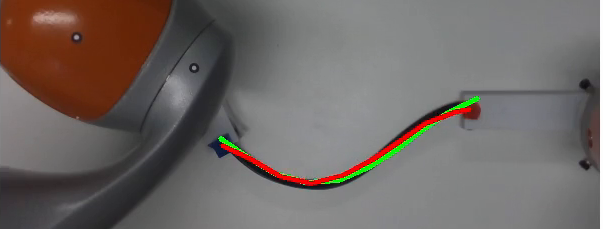
\includegraphics[width=0.45\textwidth,height=2.28cm,keepaspectratio]{conc_2f_c.png}\\
    \footnotesize Scenario 1 & \footnotesize Scenario 2\\
    \includegraphics[width=0.45\textwidth,height=2.28cm,keepaspectratio]{conc_3f_c.png} &
    \includegraphics[width=0.45\textwidth,height=2.28cm,keepaspectratio]{conc_4f_c.png}\\
    \footnotesize Scenario 3 & \footnotesize Scenario 4
  \end{tabular}
\end{frame}

\end{document}
